% ##############################################################################
\section{Mathematical Framework}
\label{sec:theory}

% ==============================================================================
\subsection{Notation and Definitions}

Let $\Omega$ denote a sample space of possible events, $\mathcal{F}$ a $\sigma$-algebra
on $\Omega$, and $P$ a probability measure. An agent $A$ at time $t$ possesses
an information set $I_{A}(t) \subseteq \mathcal{F}$ representing their knowledge.
An event $E \in \mathcal{F}$ occurs with conditional probability
$P(E \mid I_{A}(t))$.

\begin{definition}[Agent Utility]
  A utility function $U_{A}: \mathcal{F}\to \mathbb{R}$ assigns value to
  events from the perspective of agent $A$. Positive values represent
  favorable outcomes, negative values represent unfavorable outcomes,
  and zero represents neutral events.
\end{definition}

\begin{definition}[Control]
  The control function $C_{A}: \mathcal{F}\to [0,1]$ measures the degree
  to which agent $A$ causally influences event $E$. $C_{A}(E) = 0$
  indicates no control (pure chance), while $C_{A}(E) = 1$ indicates complete
  control (fully determined by agent's actions).
\end{definition}

% ==============================================================================
\subsection{Core Luck Function}

We define luck as a function of probability, utility, and control.

\begin{definition}[Luck]
  \label{def:luck} The luck experienced by agent $A$ from event $E$ is:
  \begin{equation}
    L_{A}(E) = U_{A}(E) \cdot S(E \mid I_{A}) \cdot (1 - C_{A}(E))
  \end{equation}
  where $S(E \mid I_{A})$ is the surprise function measuring the
  unexpectedness of $E$ given information $I_{A}$.
\end{definition}

The surprise function $S$ quantifies rarity. A natural choice based on information
theory is:
\begin{equation}
  S(E \mid I_{A}) = -\log P(E \mid I_{A})
\end{equation}
As illustrated in Figure~\ref{fig:surprise}, this function transforms
probability into a rarity score where rare events (low probability) receive
high surprise scores, while common events (high probability) receive
low scores. The logarithmic form ensures additivity over independent events.

\begin{figure}[H]
  \centering
  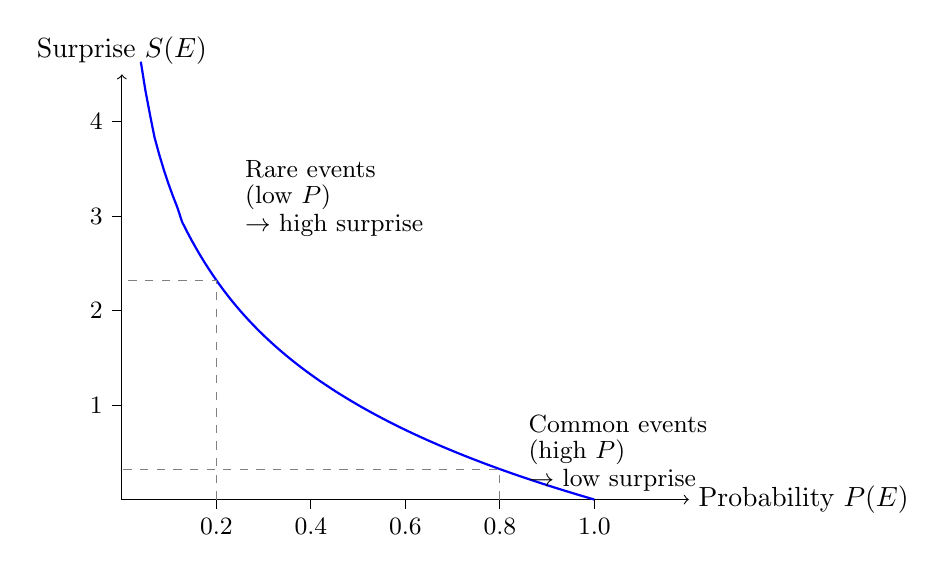
\begin{tikzpicture}[scale=1.2]
    % Axes
    \draw[->] (0,0) -- (6,0) node[right] {Probability $P(E)$};
    \draw[->] (0,0) -- (0,4.5) node[above] {Surprise $S(E)$};

    % Tick marks and labels
    \foreach \x/\label in {1/0.2, 2/0.4, 3/0.6, 4/0.8, 5/1.0}
    { \draw (\x,0) -- (\x,-0.1) node[below, font=\small] {\label}; }
    \foreach \y/\label in {1/1, 2/2, 3/3, 4/4}
    { \draw (0,\y) -- (-0.1,\y) node[left, font=\small] {\label}; }

    % The curve S = -ln(P) scaled appropriately
    \draw[thick, blue, domain=0.2:5, samples=100]
      plot
      ({\x}, {-ln(\x/5)/ln(2)});

    % Annotations
    \draw[dashed, gray]
      (1,0) --
      (1,{-ln(0.2)/ln(2)}) -- (0,{-ln(0.2)/ln(2)});
    \draw[dashed, gray]
      (4,0) --
      (4,{-ln(0.8)/ln(2)}) -- (0,{-ln(0.8)/ln(2)});

    \node[anchor=west, font=\small] at (1.2, 3.5) {Rare events};
    \node[anchor=west, font=\small] at (1.2, 3.2) {(low $P$)};
    \node[anchor=west, font=\small]
      at
      (1.2, 2.9)
      {$\rightarrow$ high surprise};

    \node[anchor=west, font=\small] at (4.2, 0.8) {Common events};
    \node[anchor=west, font=\small] at (4.2, 0.5) {(high $P$)};
    \node[anchor=west, font=\small]
      at
      (4.2, 0.2)
      {$\rightarrow$ low surprise};
  \end{tikzpicture}
  \caption{The surprise function transforms probability into a rarity score.}
  \label{fig:surprise}
\end{figure}

This formulation satisfies several desirable properties:

\begin{proposition}
  The luck function $L_{A}(E)$ is:
  \begin{enumerate}
    \item Monotonically increasing in outcome value for favorable events

    \item Monotonically decreasing in probability (rarer events are
      luckier)

    \item Monotonically decreasing in control (less controllable events
      are luckier)

    \item Zero when $U_{A}(E) = 0$ (neutral outcomes)

    \item Zero when $C_{A}(E) = 1$ (fully controlled outcomes)

    \item Information-dependent through $P(E \mid I_{A})$
  \end{enumerate}
\end{proposition}

% ==============================================================================
\subsection{Alternative Formulations}

Several variants of the core luck function address different analytical
needs.

% ------------------------------------------------------------------------------
\subsubsection{Deviation-Based Luck}

When repeated trials or comparable scenarios exist, luck can be measured
as deviation from expectation:
\begin{equation}
  L_{A}^{\text{dev}}(E) = U_{A}(E) - \mathbb{E}[U_{A}(E') \mid S_{A}]
\end{equation}
where $S_{A}$ represents the agent's strategy or controllable choices,
and the expectation is taken over events $E'$ that could occur under
that strategy. This formulation is particularly useful in skill-luck decomposition
for repeated performance evaluation.

% ------------------------------------------------------------------------------
\subsubsection{Fragility-Based Luck}

Outcomes that would change under small perturbations reflect greater
luck:
\begin{equation}
  L_{A}^{\text{frag}}(E) = U_{A}(E) \cdot \left(1 - P(E \mid \text{perturbations}
  )\right)
\end{equation}
This captures near-miss scenarios where slight differences in circumstances
would have produced substantially different outcomes.

% ------------------------------------------------------------------------------
\subsubsection{Time-Aggregated Luck}

For sequences of events over time $t = 1, \ldots, T$:
\begin{equation}
  L_{A}^{T}= \sum_{t=1}^{T}\delta^{t}L_{A}(E_{t})
\end{equation}
where $\delta \in (0,1]$ is a temporal discount factor. This formulation
addresses cumulative luck and path dependence in life trajectories.
Figure~\ref{fig:trajectories} illustrates how early luck events compound over
time through path dependence, leading to divergent cumulative outcomes. An agent
benefiting from consistent positive luck creates opportunities for further
success, while another facing compounding disadvantage from early setbacks
falls further behind. A third agent experiencing mixed luck shows limited
cumulative effect.

\begin{figure}[H]
  \centering
  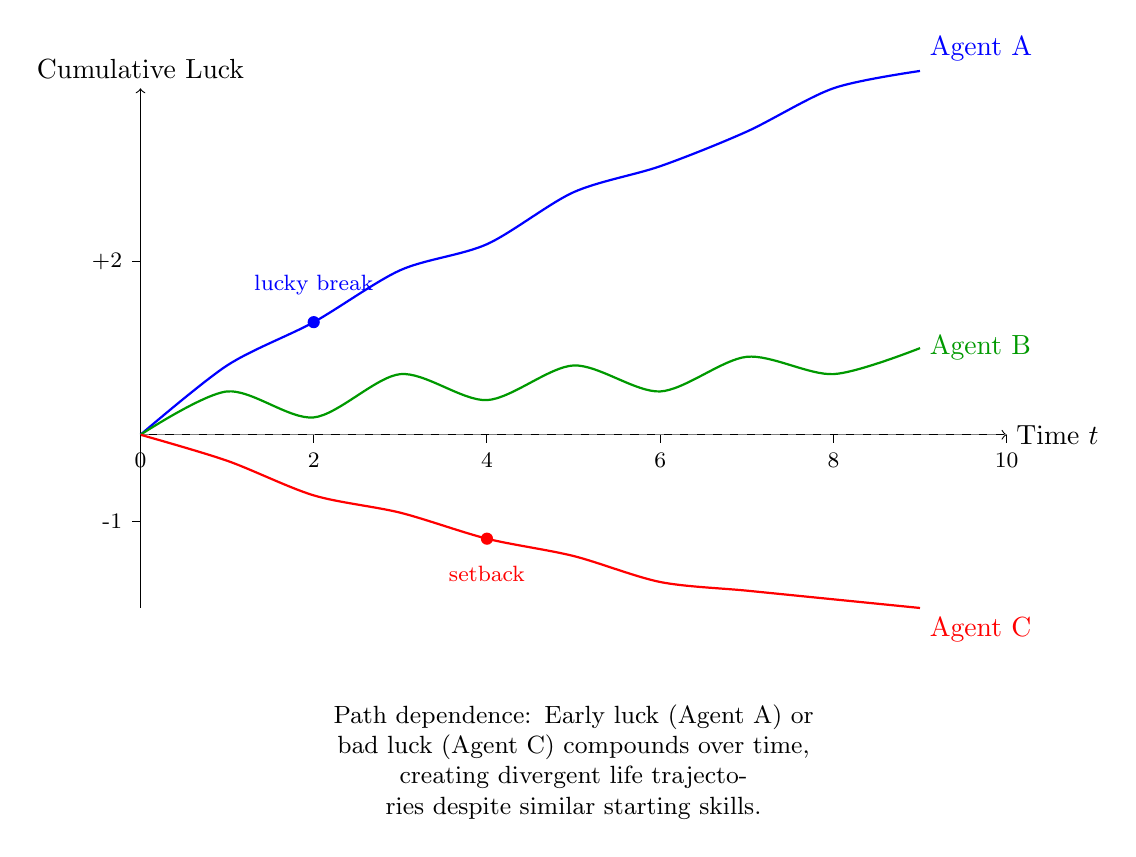
\begin{tikzpicture}[scale=1.1]
    % Axes
    \draw[->] (0,0) -- (10,0) node[right] {Time $t$};
    \draw[->] (0,-2) -- (0,4) node[above] {Cumulative Luck};
    \draw[dashed, gray] (0,0) -- (10,0);

    % Three trajectories
    % Agent A - consistently lucky
    \draw[thick, blue, smooth]
      plot
      coordinates
      { (0,0) (1,0.8) (2,1.3) (3,1.9) (4,2.2) (5,2.8) (6,3.1) (7,3.5) (8,4.0) (9,4.2) };
    \node[blue, above right] at (9,4.2) {Agent A};

    % Agent B - mixed luck
    \draw[thick, green!60!black, smooth]
      plot
      coordinates
      { (0,0) (1,0.5) (2,0.2) (3,0.7) (4,0.4) (5,0.8) (6,0.5) (7,0.9) (8,0.7) (9,1.0) };
    \node[green!60!black, right] at (9,1.0) {Agent B};

    % Agent C - consistently unlucky
    \draw[thick, red, smooth]
      plot
      coordinates
      { (0,0) (1,-0.3) (2,-0.7) (3,-0.9) (4,-1.2) (5,-1.4) (6,-1.7) (7,-1.8) (8,-1.9) (9,-2.0) };
    \node[red, below right] at (9,-2.0) {Agent C};

    % Key events marked
    \fill[blue] (2,1.3) circle (2pt);
    \node[blue, above, font=\footnotesize] at (2,1.5) {lucky break};
    \fill[red] (4,-1.2) circle (2pt);
    \node[red, below, font=\footnotesize] at (4,-1.4) {setback};

    % Time labels
    \foreach \x in {0,2,4,6,8,10}
    { \draw (\x,0) -- (\x,-0.1) node[below, font=\footnotesize] {\x}; }
    \draw (0,2) -- (-0.1,2) node[left, font=\footnotesize] {+2};
    \draw (0,-1) -- (-0.1,-1) node[left, font=\footnotesize] {-1};

    % Annotation
    \node[below, text width=9cm, align=center, font=\small]
      at
      (5,-3)
      { Path dependence: Early luck (Agent A) or bad luck (Agent C) compounds over time,\\ creating divergent life trajectories despite similar starting skills. };
  \end{tikzpicture}
  \caption{Time-aggregated luck trajectories for three agents.}
  \label{fig:trajectories}
\end{figure}

% ==============================================================================
\subsection{Skill-Luck Decomposition}

Observed outcomes $Y$ can be decomposed into skill and luck components. Let
$S_{A}$ denote the agent's strategy space and $R$ denote random variables
outside the agent's control.

\begin{definition}[Expected Performance]
  The skill-based expected outcome is:
  \begin{equation}
    \bar{Y}_{A}= \mathbb{E}[Y \mid S_{A}, I_{A}]
  \end{equation}
\end{definition}

\begin{definition}[Luck Component]
  The luck component of outcome $Y$ is:
  \begin{equation}
    L_{A}(Y) = Y - \bar{Y}_{A}
  \end{equation}
\end{definition}

This decomposition enables performance evaluation that accounts for uncontrollable
factors. In contexts with repeated observations, the variance of outcomes
can be partitioned:
\begin{equation}
  \text{Var}(Y) = \text{Var}(\bar{Y}_{A}) + \text{Var}(L_{A}(Y))
\end{equation}
where $\text{Var}(\bar{Y}_{A})$ represents skill-based variation and
$\text{Var}(L_{A}(Y))$ represents luck-based variation.
Figure~\ref{fig:decomposition} illustrates this decomposition: expected outcomes
$\bar{Y}_{A}$ and $\bar{Y}_{B}$ reflect skill differences, while actual outcomes
$Y_{A}$ and $Y_{B}$ deviate due to luck. Notably, an agent with lower skill
can outperform a higher-skilled agent through favorable luck, though this
becomes less likely as skill differences increase.

\begin{figure}[H]
  \centering
  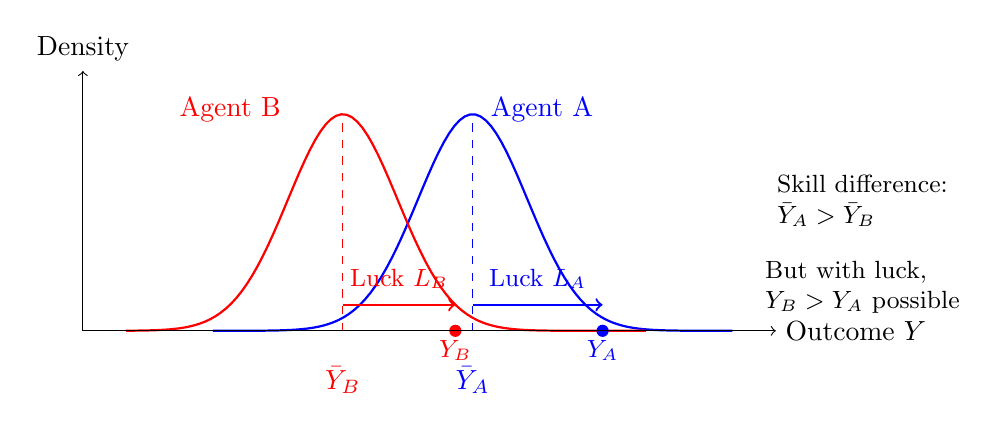
\begin{tikzpicture}[scale=1.1]
    % Draw normal distribution curves
    % Agent A - higher skill
    \draw[thick, blue, domain=-2:4, samples=100]
      plot
      ({\x}, {2.5*exp(-(\x-1)^2/0.8)});
    \draw[dashed, blue] (1,0) -- (1,2.5);
    \node[blue, below] at (1,-0.3) {$\bar{Y}_{A}$};
    \node[blue, above] at (1.8,2.3) {Agent A};

    % Agent B - lower skill
    \draw[thick, red, domain=-3:3, samples=100]
      plot
      ({\x}, {2.5*exp(-(\x+0.5)^2/0.8)});
    \draw[dashed, red] (-0.5,0) -- (-0.5,2.5);
    \node[red, below] at (-0.5,-0.3) {$\bar{Y}_{B}$};
    \node[red, above] at (-1.8,2.3) {Agent B};

    % Actual outcomes
    \draw[->, thick, blue] (1,0.3) -- (2.5,0.3);
    \node[blue, font=\small] at (1.75, 0.6) {Luck $L_{A}$};
    \fill[blue] (2.5,0) circle (2pt) node[below, font=\small] {$Y_{A}$};

    \draw[->, thick, red] (-0.5,0.3) -- (0.8,0.3);
    \node[red, font=\small] at (0.15, 0.6) {Luck $L_{B}$};
    \fill[red] (0.8,0) circle (2pt) node[below, font=\small] {$Y_{B}$};

    % Axes
    \draw[->] (-3.5,0) -- (4.5,0) node[right] {Outcome $Y$};
    \draw[->] (-3.5,0) -- (-3.5,3) node[above] {Density};

    % Annotation
    \node[align=left, font=\small]
      at
      (5.5, 1.5)
      {Skill difference:\\$\bar{Y}_{A}> \bar{Y}_{B}$};
    \node[align=left, font=\small]
      at
      (5.5, 0.5)
      {But with luck,\\$Y_{B}> Y_{A}$ possible};
  \end{tikzpicture}
  \caption{Skill-luck decomposition for two agents.}
  \label{fig:decomposition}
\end{figure}

% ==============================================================================
\subsection{Axioms and Properties}

The framework rests on several axioms that formalize intuitive
properties of luck:

\begin{assumption}
  [Neutrality] Outcomes with zero utility contribute zero luck:
  $U_{A}(E) = 0 \implies L_{A}(E) = 0$.
\end{assumption}

\begin{assumption}
  [Control Dominance] Fully controlled outcomes are not lucky:
  $C_{A}(E) = 1 \implies L_{A}(E) = 0$.
\end{assumption}

\begin{assumption}
  [Information Dependence] Luck depends on the agent's prior information:
  $L_{A}(E)$ is a function of $P(E \mid I_{A})$ rather than $P(E)$ alone.
\end{assumption}

\begin{assumption}
  [Value Monotonicity] For events with equal probability and control,
  luck increases with absolute utility: if $P(E_{1}\mid I_{A}) = P(E_{2}\mid
  I_{A})$ and $C_{A}(E_{1}) = C_{A}(E_{2})$, then
  $|L_{A}(E_{1})| < |L_{A}(E_{2})|$ when
  $|U_{A}(E_{1})| < |U_{A}(E_{2})|$.
\end{assumption}

% ##############################################################################
\section{Event Rating and Measurement}
\label{sec:rating}

% ==============================================================================
\subsection{Rating Pipeline}

Practical application of the framework requires a systematic procedure
for rating events. We propose a step-by-step pipeline illustrated in
Figure~\ref{fig:pipeline}. The seven-step procedure transforms raw event
information into a normalized luck score suitable for cross-agent and
cross-event comparison.

% TODO(gp): Improve this picture using mermaid or graphviz
\begin{figure}[H]
  \centering
  \begin{tikzpicture}[
    node distance=1.2cm,
    stepnode/.style={rectangle, draw, fill=blue!15, text width=3.5cm, minimum height=0.9cm, align=center, font=\small},
    decision/.style={diamond, draw, fill=orange!15, text width=2cm, minimum height=0.8cm, align=center, font=\small},
    arrow/.style={->, >=stealth, thick}
  ]
    % Steps
    \node[stepnode] (step1) {1. Specify Agent \& Event\\$A$, $E$, $t$};
    \node[stepnode, below of=step1]
      (step2)
      {2. Define Reference Model\\$P(\cdot|I_{A}(t))$};
    \node[stepnode, below of=step2]
      (step3)
      {3. Compute Surprise\\$S(E) = -\log P(E|I_{A})$};
    \node[stepnode, below of=step3]
      (step4)
      {4. Assess Utility\\$U_{A}(E)$};
    \node[stepnode, below of=step4]
      (step5)
      {5. Estimate Control\\$C_{A}(E) \in [0,1]$};
    \node[stepnode, below of=step5]
      (step6)
      {6. Calculate Luck\\$L_{A}(E) = U_{A}\cdot S \cdot (1-C_{A})$};
    \node[stepnode, below of=step6, fill=green!15]
      (step7)
      {7. Normalize\\$L_{A}^{*}(E)$ (z-score)};

    % Arrows
    \draw[arrow] (step1) -- (step2);
    \draw[arrow] (step2) -- (step3);
    \draw[arrow] (step3) -- (step4);
    \draw[arrow] (step4) -- (step5);
    \draw[arrow] (step5) -- (step6);
    \draw[arrow] (step6) -- (step7);

    % Side annotations
    \node[
      right=0.5cm of step2,
      text width=3cm,
      font=\footnotesize,
      align=left
    ] {Base rates, models, forecasts};
    \node[
      right=0.5cm of step4,
      text width=3cm,
      font=\footnotesize,
      align=left
    ] {Money, health, career metrics};
    \node[
      right=0.5cm of step5,
      text width=3cm,
      font=\footnotesize,
      align=left
    ] {Causal analysis, variance decomp};
    \node[
      right=0.5cm of step7,
      text width=3cm,
      font=\footnotesize,
      align=left
    ] {Compare across agents/events};
  \end{tikzpicture}
  \caption{Event rating pipeline.}
  \label{fig:pipeline}
\end{figure}

% ------------------------------------------------------------------------------
\subsubsection{Step 1: Specify Agent and Event}

Clearly identify the agent $A$, the event $E$, and the time $t$ at which
the event occurs. Luck is agent-relative and context-dependent.

% ------------------------------------------------------------------------------
\subsubsection{Step 2: Define Reference Model}

Construct a probability model $P(\cdot \mid I_{A}(t))$ representing the agent's
information state prior to the event. This may involve:
\begin{itemize}
  \item Historical base rates for similar events

  \item Statistical models fitted to relevant data

  \item Expert forecasts or prediction markets

  \item Agent-specific models accounting for their knowledge and position
\end{itemize}

% ------------------------------------------------------------------------------
\subsubsection{Step 3: Compute Surprise}

Calculate the surprise score:
\begin{equation}
  S(E) = -\log P(E \mid I_{A})
\end{equation}
Low-probability events receive higher surprise scores.

% ------------------------------------------------------------------------------
\subsubsection{Step 4: Assess Outcome Value}

Determine utility $U_{A}(E)$ using appropriate scales:
\begin{itemize}
  \item Monetary value for financial outcomes

  \item Health metrics (life expectancy, quality-adjusted life years)
    for health outcomes

  \item Career advancement measures for professional outcomes

  \item Normalized scores for comparative analysis
\end{itemize}

% ------------------------------------------------------------------------------
\subsubsection{Step 5: Estimate Control}

Quantify the degree of agent control $C_{A}(E) \in [0,1]$. Methods include:
\begin{itemize}
  \item Causal modeling to identify controllable versus uncontrollable factors

  \item Variance decomposition showing proportion explained by agent's actions

  \item Counterfactual analysis examining outcome sensitivity to agent's
    choices

  \item Repeatability analysis measuring consistency of outcomes across similar
    scenarios
\end{itemize}

% ------------------------------------------------------------------------------
\subsubsection{Step 6: Calculate Luck Score}

Apply the luck function:
\begin{equation}
  L_{A}(E) = U_{A}(E) \cdot S(E) \cdot (1 - C_{A}(E))
\end{equation}

% ------------------------------------------------------------------------------
\subsubsection{Step 7: Normalize}

For cross-event or cross-agent comparison, normalize within relevant
populations:
\begin{equation}
  L_{A}^{*}(E) = \frac{L_{A}(E) - \mu_{L}}{\sigma_{L}}
\end{equation}
producing a standardized luck z-score.

% ==============================================================================
\subsection{Data Requirements}

Empirical application requires several types of data:

\begin{table}[H]
  \centering
  \begin{tabular}{ll}
    \toprule \textbf{Data Type} & \textbf{Purpose}               \\
    \midrule Probability data   & Estimate $P(E \mid I_{A})$     \\
    Historical frequencies      & Base rates for similar events  \\
    Information records         & Define information set $I_{A}$ \\
    Outcome measurements        & Quantify utility $U_{A}(E)$    \\
    Decision logs               & Track controllable actions     \\
    Causal data                 & Estimate control $C_{A}(E)$    \\
    Baseline performance        & Compute expected values        \\
    Population distributions    & Normalize luck scores          \\
    \bottomrule
  \end{tabular}
  \caption{Data requirements for empirical luck measurement}
  \label{tab:data}
\end{table}

% ==============================================================================
\subsection{Example Application}

Consider a concrete example: an entrepreneur's startup succeeds after raising
venture capital. We analyze the luck component:

\begin{itemize}
  \item \textbf{Event:} Startup achieves successful exit within five
    years

  \item \textbf{Probability:} Base rate for similar ventures is
    approximately 10\%, so $P(E) = 0.1$ and
    $S(E) = -\log(0.1) \approx 2.3$

  \item \textbf{Utility:} Financial gain of \$5M, normalized to
    $U_{A}(E) = 5$

  \item \textbf{Control:} Entrepreneur's strategy and execution
    contributed substantially, but market conditions and network effects
    were also crucial; estimate $C_{A}(E) = 0.6$

  \item \textbf{Luck Score:}
    $L_{A}(E) = 5 \times 2.3 \times (1 - 0.6) = 4.6$
\end{itemize}

This positive luck score indicates that while the entrepreneur's skill was
important, favorable circumstances and timing contributed significantly
to the outcome. Figure~\ref{fig:example} visualizes the calculation,
decomposing the entrepreneur's success into components: surprise from low
base rate ($P=0.1$), high financial utility (\$5M normalized to 5), and
moderate lack of control (0.4, since skill $C=0.6$ was important). The
resulting luck score of 4.6 indicates substantial favorable luck.

\begin{figure}[H]
  \centering
  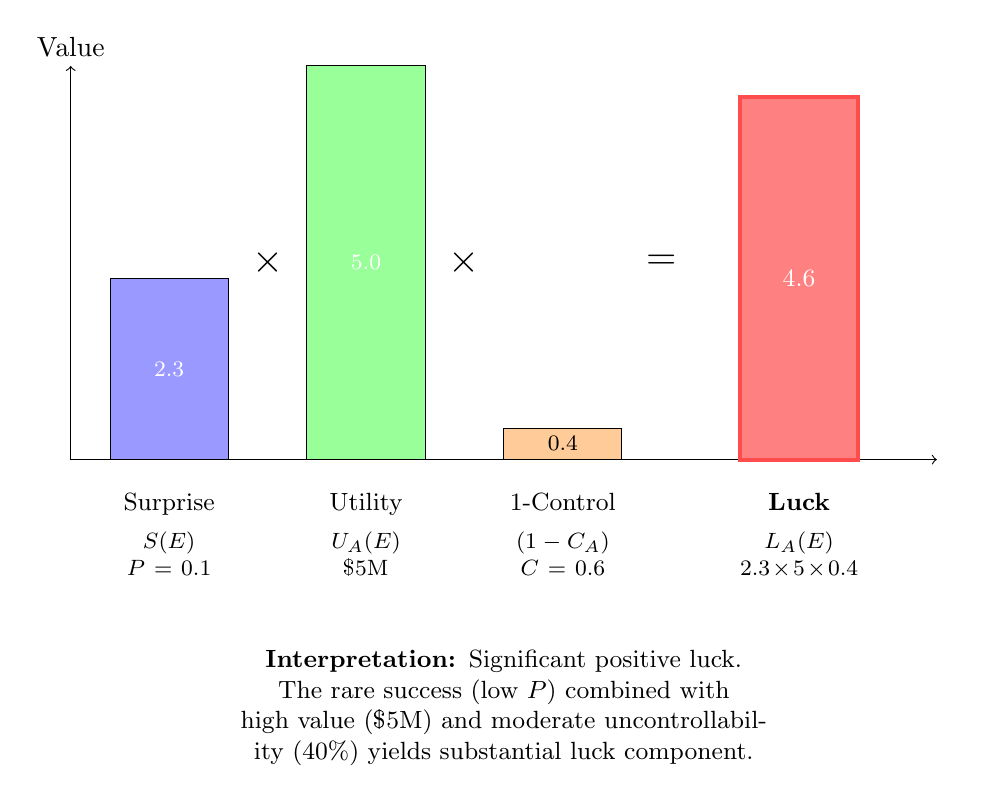
\begin{tikzpicture}[scale=1.0]
    % Bar chart
    \draw[->] (0,0) -- (0,5) node[above] {Value};
    \draw[->] (0,0) -- (11,0) node[right] {};

    % Bars
    % Probability/Surprise
    \draw[fill=blue!40]
      (0.5,0) rectangle (2,2.3)
      node[midway, white, font=\footnotesize] {2.3};
    \node[below, font=\small] at (1.25,-0.3) {Surprise};
    \node[below, font=\footnotesize, text width=1.5cm, align=center]
      at
      (1.25,-0.8)
      {$S(E)$\\$P=0.1$};

    % Utility
    \draw[fill=green!40]
      (3,0) rectangle (4.5,5)
      node[midway, white, font=\footnotesize] {5.0};
    \node[below, font=\small] at (3.75,-0.3) {Utility};
    \node[below, font=\footnotesize, text width=1.5cm, align=center]
      at
      (3.75,-0.8)
      {$U_{A}(E)$\\\$5M};

    % Control
    \draw[fill=orange!40]
      (5.5,0) rectangle (7,0.4)
      node[midway, font=\footnotesize] {0.4};
    \node[below, font=\small] at (6.25,-0.3) {1-Control};
    \node[below, font=\footnotesize, text width=1.5cm, align=center]
      at
      (6.25,-0.8)
      {$(1-C_{A})$\\$C=0.6$};

    % Result
    \draw[fill=red!50, draw=red!70, line width=1.5pt]
      (8.5,0) rectangle (10,4.6);
    \node[white, font=\small] at (9.25,2.3) {4.6};
    \node[below, font=\small] at (9.25,-0.3) {\textbf{Luck}};
    \node[below, font=\footnotesize, text width=1.5cm, align=center]
      at
      (9.25,-0.8)
      {$L_{A}(E)$\\$2.3 \times 5 \times 0.4$};

    % Multiplication signs
    \node[font=\Large] at (2.5,2.5) {$\times$};
    \node[font=\Large] at (5,2.5) {$\times$};
    \node[font=\Large] at (7.5,2.5) {$=$};

    % Interpretation
    \node[below, text width=10cm, align=center, font=\small]
      at
      (5.5,-2.3)
      { \textbf{Interpretation:} Significant positive luck. The rare success (low $P$) combined with\\ high value (\$5M) and moderate uncontrollability (40\%) yields substantial luck component. };
  \end{tikzpicture}
  \caption{Startup example calculation.}
  \label{fig:example}
\end{figure}

% ##############################################################################
\section{Societal Modeling and Aggregate Measures}
\label{sec:society}

% ==============================================================================
\subsection{Modeling Life Outcomes}

To analyze luck at the societal level, we model individual life outcomes
as a function of three input categories:

\begin{itemize}
  \item \textbf{Circumstances} $B_{i}$: Factors not chosen by the individual
    (parental background, birth location, cohort, genetics)

  \item \textbf{Choices} $A_{i}$: Factors under individual control (effort,
    decisions, strategies)

  \item \textbf{Shocks} $S_{i}$: Random events affecting the individual (accidents,
    encounters, policy changes)
\end{itemize}

A general outcome model takes the form:
\begin{equation}
  Y_{i}= f(B_{i}, A_{i}) + g(S_{i}) + \varepsilon_{i}
\end{equation}
where $f$ represents the deterministic relationship between
circumstances, choices, and outcomes, $g$ captures the effect of random shocks,
and $\varepsilon_{i}$ represents measurement error or small unmodeled
factors. Figure~\ref{fig:causal} visualizes this model: circumstances $B_{i}$
(unearned advantages) and choices $A_{i}$ (agency) jointly determine expected
outcomes, while shocks $S_{i}$ (random events) introduce luck. Circumstances
also constrain available choices. The variance decomposition separates
skill-based from luck-based variation in outcomes.

% TODO(ai_gp): Convert this picture in graphviz
\begin{figure}[H]
  \centering
  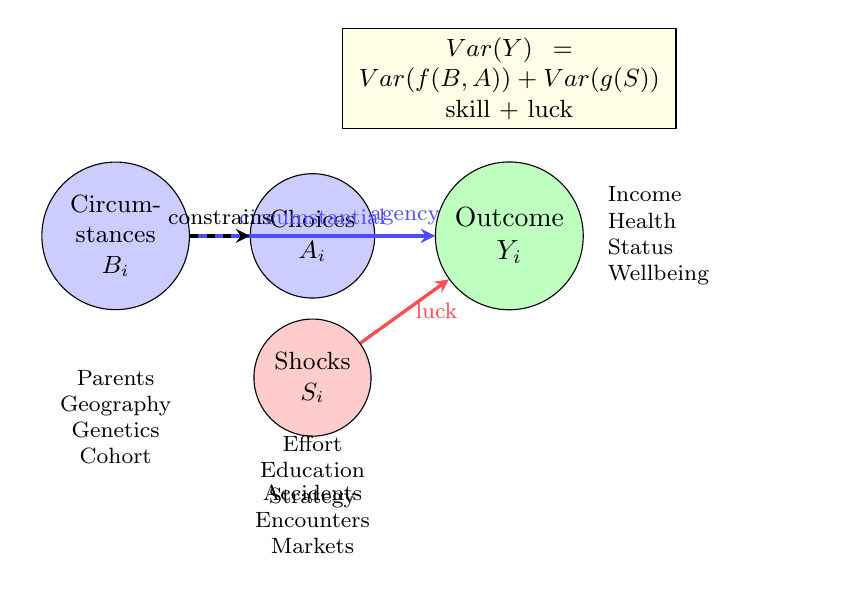
\begin{tikzpicture}[
    node distance=2.5cm and 2cm,
    varnode/.style={circle, draw, fill=blue!20, minimum size=1.3cm, align=center, font=\small},
    outcome/.style={circle, draw, fill=green!25, minimum size=1.5cm, align=center, font=\normalsize},
    shock/.style={circle, draw, fill=red!20, minimum size=1.3cm, align=center, font=\small},
    arrow/.style={->, >=stealth, very thick}
  ]
    % Nodes
    \node[varnode] (B) {Circum-\\stances\\$B_{i}$};
    \node[varnode, right of=B] (A) {Choices\\$A_{i}$};
    \node[shock, below of=A, node distance=1.8cm] (S) {Shocks\\$S_{i}$};
    \node[outcome, right of=A] (Y) {Outcome\\$Y_{i}$};

    % Arrows
    \draw[arrow, blue!70]
      (B) -- (Y)
      node[midway, above, font=\footnotesize] {circumstantial};
    \draw[arrow, blue!70]
      (A) -- (Y)
      node[midway, above, font=\footnotesize] {agency};
    \draw[arrow, red!70]
      (S) -- (Y)
      node[midway, right, font=\footnotesize] {luck};
    \draw[arrow, dashed]
      (B) -- (A)
      node[midway, above, font=\footnotesize] {constrains};

    % Annotations
    \node[
      below of=B,
      node distance=2.3cm,
      text width=2cm,
      align=center,
      font=\footnotesize
    ] {Parents\\Geography\\Genetics\\Cohort};
    \node[
      below of=A,
      node distance=3cm,
      text width=2cm,
      align=center,
      font=\footnotesize
    ] {Effort\\Education\\Strategy};
    \node[
      below of=S,
      node distance=1.8cm,
      text width=2cm,
      align=center,
      font=\footnotesize
    ] {Accidents\\Encounters\\Markets};
    \node[
      right of=Y,
      node distance=2.5cm,
      text width=2.5cm,
      align=left,
      font=\footnotesize
    ] {Income\\Health\\Status\\Wellbeing};

    % Variance decomposition annotation
    \node[
      above of=Y,
      node distance=2cm,
      text width=4cm,
      align=center,
      font=\small,
      draw,
      fill=yellow!10
    ]
      { $\text{Var}(Y) = \text{Var}(f(B,A)) + \text{Var}(g(S))$\\ skill + luck };
  \end{tikzpicture}
  \caption{Causal model of societal outcomes.}
  \label{fig:causal}
\end{figure}

% ==============================================================================
\subsection{Individual Luck Measures}

Three complementary measures capture different aspects of luck:

% ------------------------------------------------------------------------------
\subsubsection{Residual Luck}

Residual luck measures the deviation of actual outcomes from predictions
based on circumstances and choices:
\begin{equation}
  L_{i}^{\text{res}}= Y_{i}- \mathbb{E}[Y_{i}\mid B_{i}, A_{i}]
\end{equation}
This represents the core luck component—the portion of outcomes not
explained by observable inputs.

% ------------------------------------------------------------------------------
\subsubsection{Surprise-Weighted Luck}

For outcomes far from expectations, surprise weighting emphasizes
extreme cases:
\begin{equation}
  L_{i}^{\text{sur}}= U(Y_{i}) \cdot \left[-\log P(Y_{i}\mid B_{i}, A_{i}
  )\right]
\end{equation}

% ------------------------------------------------------------------------------
\subsubsection{Control-Adjusted Luck}

When control varies across individuals or contexts:
\begin{equation}
  L_{i}^{\text{ctrl}}= (Y_{i}- \mathbb{E}[Y_{i}\mid B_{i}, A_{i}]) \cdot
  (1 - C_{i})
\end{equation}
where $C_{i}$ represents the degree of control individual $i$ has over
their outcomes.

% ==============================================================================
\subsection{Aggregate Luck Metrics}

Societal-level analysis aggregates individual luck scores to characterize
distributional properties.

% ------------------------------------------------------------------------------
\subsubsection{Luck Inequality}

The Gini coefficient of absolute luck values measures dispersion:
\begin{equation}
  G_{L}= \frac{\sum_{i=1}^{n}\sum_{j=1}^{n}|L_{i}- L_{j}|}{2n^{2}\bar{L}}
\end{equation}
High luck inequality indicates that some individuals experience far more
favorable or unfavorable luck than others.

% ------------------------------------------------------------------------------
\subsubsection{Circumstantial Dependence}

The proportion of outcome variance explained by circumstances (rather than
choices or luck) measures the degree to which outcomes are predetermined
by birth:
\begin{equation}
  \rho_{B}= \frac{\text{Var}(\mathbb{E}[Y \mid B])}{\text{Var}(Y)}
\end{equation}
Higher values indicate less social mobility and greater importance of circumstantial
luck.

% ------------------------------------------------------------------------------
\subsubsection{Agency Contribution}

The additional variance explained by choices beyond circumstances:
\begin{equation}
  \rho_{A}= \frac{\text{Var}(\mathbb{E}[Y \mid B, A]) - \text{Var}(\mathbb{E}[Y
  \mid B])}{\text{Var}(Y)}
\end{equation}
This measures the role of individual agency in determining outcomes.

% ------------------------------------------------------------------------------
\subsubsection{Mobility Index}

Intergenerational mobility can be measured through the correlation
between parent and child outcomes:
\begin{equation}
  M = 1 - \text{Corr}(Y_{\text{parent}}, Y_{\text{child}})
\end{equation}
Lower correlation (higher $M$) suggests that circumstances of birth have
less influence on eventual outcomes.

% ==============================================================================
\subsection{Empirical Estimation}

Practical estimation typically proceeds through regression-based
variance decomposition. Consider a model:
\begin{equation}
  Y_{i}= \alpha + \beta_{B}B_{i}+ \beta_{A}A_{i}+ \varepsilon_{i}
\end{equation}

Stepwise regression allows decomposition:
\begin{enumerate}
  \item Regress $Y$ on $B$ alone: variance explained is $R^{2}_{B}$

  \item Regress $Y$ on both $B$ and $A$: variance explained is
    $R^{2}_{B,A}$

  \item Residual variance: $1 - R^{2}_{B,A}$ represents luck

  \item Agency contribution: $R^{2}_{B,A}- R^{2}_{B}$
\end{enumerate}
Figure~\ref{fig:variance} compares variance decomposition in two stylized
societies. The low mobility society (left) shows outcome variance dominated
by circumstances of birth ($\rho_{B}= 0.60$), with limited role for agency
($\rho_{A}= 0.20$). The high mobility society (right) exhibits lower
circumstantial dependence ($\rho_{B}= 0.30$) and greater agency contribution
($\rho_{A}= 0.40$). Both societies contain irreducible luck components from
random shocks.

\begin{figure}[H]
  \centering
  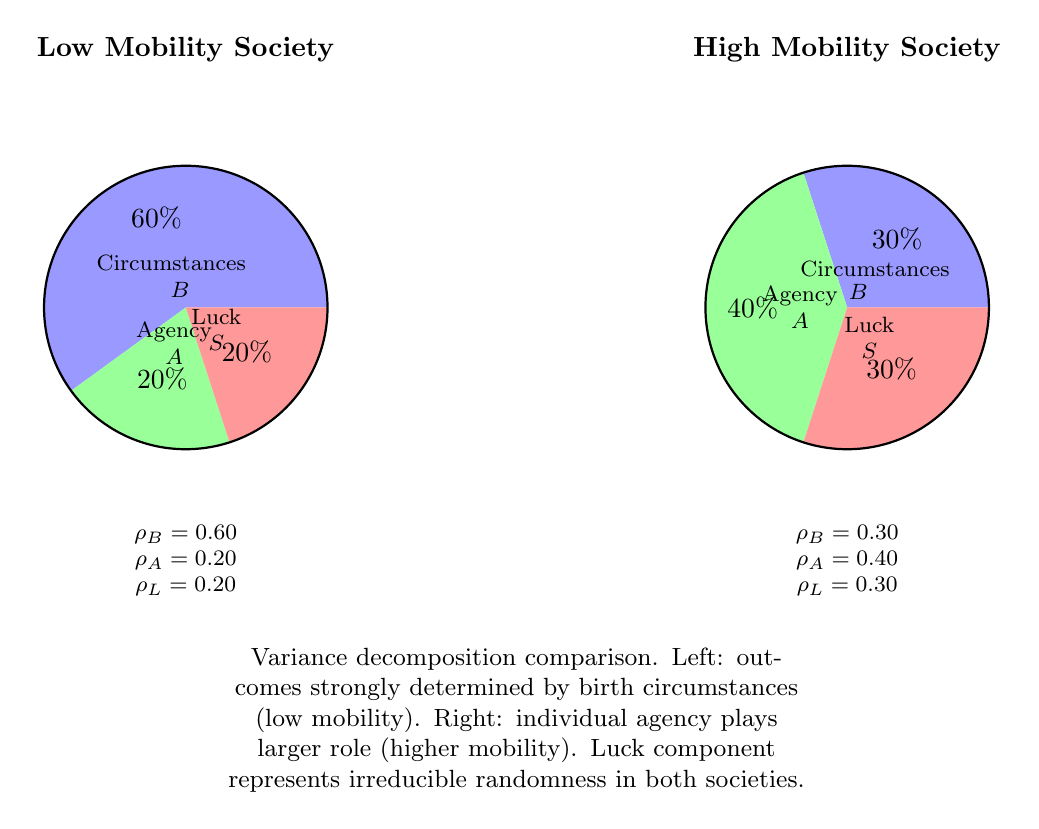
\begin{tikzpicture}[scale=1.2]
    % Two pie charts comparing societies

    % Society 1 - High circumstantial dependence
    \begin{scope}[xshift=0cm]
      \node[above] at (0,2.5) {\textbf{Low Mobility Society}};

      % Pie chart
      \fill[blue!40] (0,0) -- (0:1.5) arc (0:216:1.5) -- cycle;
      \fill[green!40] (0,0) -- (216:1.5) arc (216:288:1.5) -- cycle;
      \fill[red!40] (0,0) -- (288:1.5) arc (288:360:1.5) -- cycle;

      \draw[thick] (0,0) circle (1.5);

      % Labels with percentages
      \node at (108:1) {60\%};
      \node[font=\footnotesize] at (108:0.5) {Circumstances};
      \node[font=\footnotesize] at (108:0.2) {$B$};

      \node at (252:0.8) {20\%};
      \node[font=\footnotesize, text width=1.5cm, align=center]
        at
        (252:0.4)
        {Agency\\$A$};

      \node at (324:0.8) {20\%};
      \node[font=\footnotesize, text width=1.2cm, align=center]
        at
        (324:0.4)
        {Luck\\$S$};

      % Metrics below
      \node[below, align=center, font=\footnotesize]
        at
        (0,-2.2)
        { $\rho_{B}= 0.60$\\ $\rho_{A}= 0.20$\\ $\rho_{L}= 0.20$ };
    \end{scope}

    % Society 2 - More mobility
    \begin{scope}[xshift=7cm]
      \node[above] at (0,2.5) {\textbf{High Mobility Society}};

      % Pie chart
      \fill[blue!40] (0,0) -- (0:1.5) arc (0:108:1.5) -- cycle;
      \fill[green!40] (0,0) -- (108:1.5) arc (108:252:1.5) -- cycle;
      \fill[red!40] (0,0) -- (252:1.5) arc (252:360:1.5) -- cycle;

      \draw[thick] (0,0) circle (1.5);

      % Labels with percentages
      \node at (54:0.9) {30\%};
      \node[font=\footnotesize] at (54:0.5) {Circumstances};
      \node[font=\footnotesize] at (54:0.2) {$B$};

      \node at (180:1) {40\%};
      \node[font=\footnotesize, text width=1.5cm, align=center]
        at
        (180:0.5)
        {Agency\\$A$};

      \node at (306:0.8) {30\%};
      \node[font=\footnotesize, text width=1.2cm, align=center]
        at
        (306:0.4)
        {Luck\\$S$};

      % Metrics below
      \node[below, align=center, font=\footnotesize]
        at
        (0,-2.2)
        { $\rho_{B}= 0.30$\\ $\rho_{A}= 0.40$\\ $\rho_{L}= 0.30$ };
    \end{scope}

    % Legend
    \node[below, text width=12cm, align=center, font=\small]
      at
      (3.5,-3.5)
      { Variance decomposition comparison. Left: outcomes strongly determined by birth circumstances\\ (low mobility). Right: individual agency plays larger role (higher mobility). Luck component\\ represents irreducible randomness in both societies. };
  \end{tikzpicture}
  \caption{Variance decomposition in two stylized societies.}
  \label{fig:variance}
\end{figure}
